\chapter{Разработка метода решения задачи} \label{ch3}
	
\section{Измерение инфракрасного излучения} \label{ch3:sec1}

Все объекты, температура которых превышает температуру абсолютного нуля излучают электромагнитное тепловое излучение. Согласно распределению длин волн, излучаемая энергия имеет зависимость от температуры поверхности объекта, которую можно описать законом излучения Планка:
\begin{equation} 
M(\lambda, T)=\frac{c_1 \lambda^{-5}}{\mathrm{e}^{c_2 / \lambda T}-1}
\end{equation} 
где $M(\lambda, T)$ величина излучения абсолютно черного тела. $c_1$ и $c_2$ первая и вторая константы излучения соответственно. $\lambda$ длина волны излучения и $T$ абсолютная температура черного тела. Когда $\exp \left(c_2 / \lambda T\right)>>1$, формулу Планка можно заменить следующей формулой смещения Вина:
\begin{equation} 
M_{\mathrm{b}}(\lambda, T)=c_1 \lambda^{-5} \mathrm{e}^{-c_2 / \lambda T}
\end{equation} 

Закон смещения Вина указывает на то, что чем выше температура объекта, тем короче длина волны его спектра излучения, и центральный пик смещается в сторону коротких волн. Однако излучаемая энергия, поступающая на чувствительную поверхность датчика, в реальных измерениях включает не только излучаемую энергию целевого объекта, но также энергию окружающих объектов и атмосферы. Поэтому спектральную излучательную способность поверхности целевого объекта можно выразить следующим образом:
\begin{equation} 
L_\lambda=\varepsilon_\lambda M_{\mathrm{b}}\left(\lambda, T_{\mathrm{obj}}\right)+\left(1-\alpha_\lambda\right) M_{\mathrm{b}}\left(\lambda, T_{\mathrm{sur}}\right)
\end{equation} 
где $\varepsilon_\lambda$ и $T_{\mathrm{obj}}$ излучательная способность и температура целевого объекта соответсвенно; $\varepsilon_\lambda M_b\left(\lambda, T_{\mathrm{obj}}\right)$ и $M_b(\lambda$, $T_{sur}$) это спектральная яркость целевого объекта и окружающей среды. $\alpha_\lambda$ поглощающая способность поверхности целевого объекта. $T_{\mathrm{sur}}$ температура окружающей среды.

Первый множитель в правой части уравнения (3.3) представляет собой спектральную яркость поверхности целевого объекта, а второй множитель — спектральную яркость окружающей среды, отраженную от целевого объекта. Излучение, действующее на систему измерения инфракрасного излучения, представлено на рисунке \ref{scheme}, основными источниками которого являются окружающая среда, объект и атмосфера. Это может быть выражено как:
\begin{equation} 
\begin{multlined}
E_\lambda=A_{\mathrm{obj}} d^{-2}\left[\tau_{\alpha \lambda} \varepsilon_\lambda M_{\mathrm{b}}\left(\lambda, T_{\mathrm{obj}}\right)+\tau_{\mathrm{a} \lambda}\left(1-\alpha_\lambda\right) \cdot M_{\mathrm{b}}\left(\lambda, T_{\mathrm{sur}}\right)+ \\ \varepsilon_{\alpha \lambda} M_{\mathrm{b}}\left(\lambda, T_{\mathrm{atm}}\right)\right]
\end{multlined}
\end{equation} 

\begin{figure}[ht!]
    \centering
    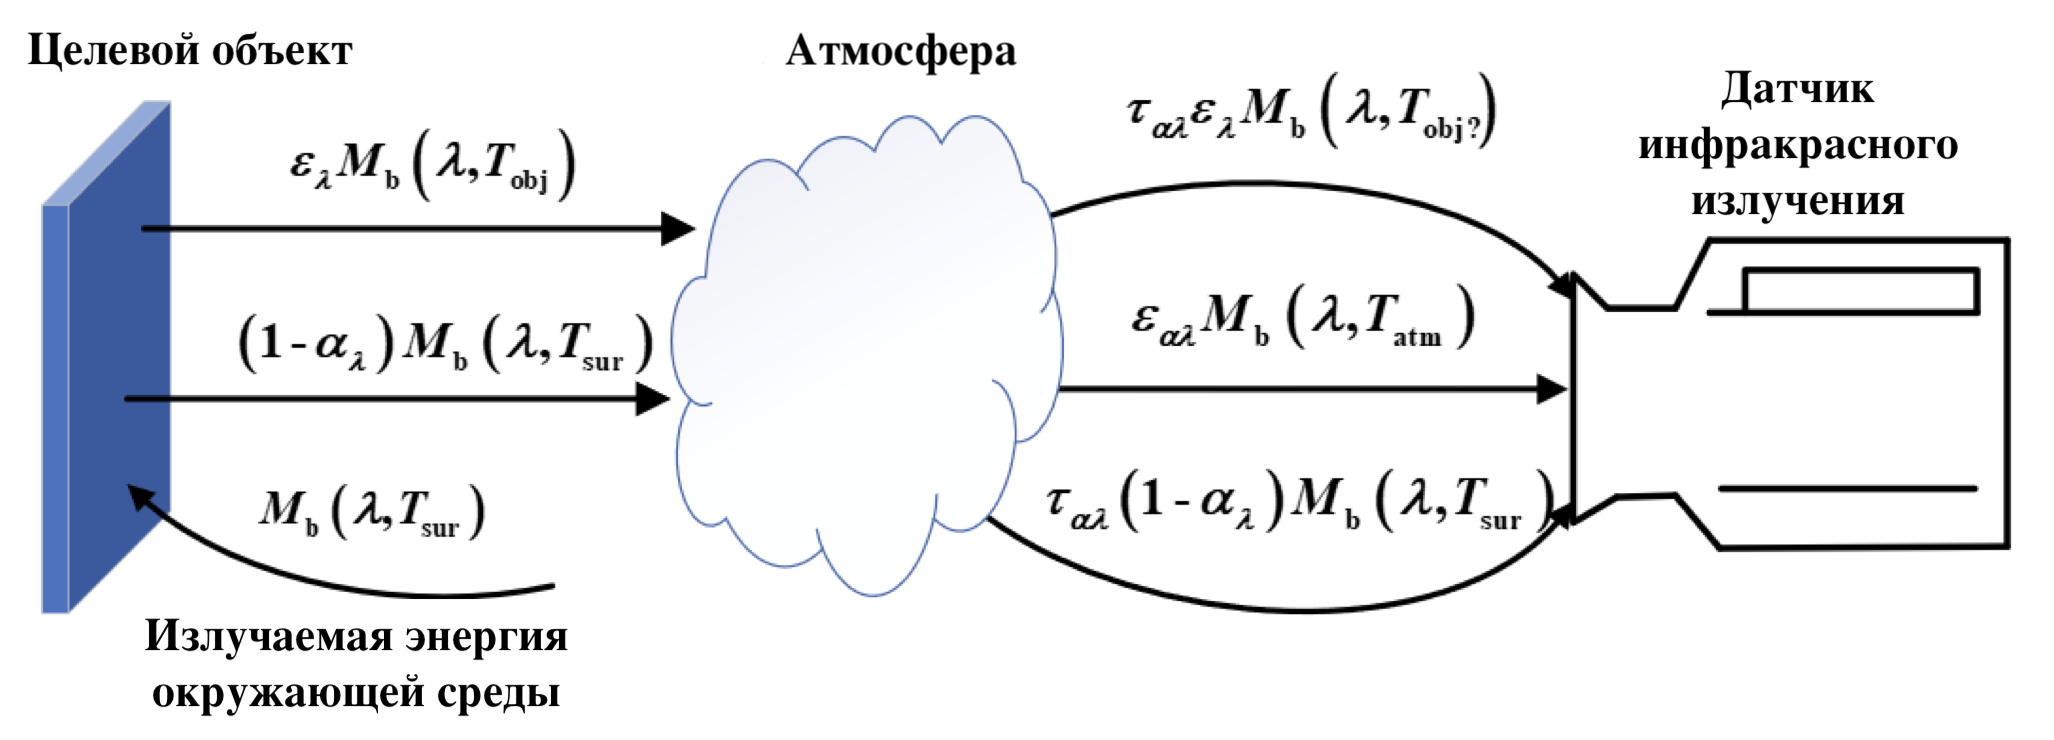
\includegraphics[width=0.8\linewidth]{my_folder/images/infr-scheme.png}
    \caption{Принципиальная схема получаемой энергии системы измерения инфракрасного излучения}
    \label{scheme}
\end{figure}
где $A_{\text{obj}}$ — видимая площадь целевого объекта, соответствующая минимальному углу тензора датчика инфракрасного изслучения, а $d$ — расстояние от целевого объекта до датчика инфракрасного излучения. В общем случае $\mathrm{A}_{\mathrm{obj}} d^{-2}$ является константой. $\tau_{\alpha \lambda}, \varepsilon_{\alpha \lambda} \mathrm{M}_{\mathrm{b}}\left(\lambda, T_{\mathrm{atm}}\right), \varepsilon_{\alpha \lambda}$ и $T_{\mathrm{atm}}$ — это спектральная пропускная способность, излучение, коэффициент излучения и температура атмосферы соответственно.

Полученная инфракрасная излучаемая энергия преобразуется датчиком в сигнал тока, то есть падающая инфракрасная излучаемая энергия интегрируется по полосе пропускания $\Delta \lambda$. Следовательно, зависимость между излучаемой энергией и током можно выразить следующим образом:
\begin{equation} 
I_0 = \int_{\Delta \lambda} A_{\mathrm{R}} R_\lambda E_\lambda \tau_{\mathrm{f}} \mathrm{d} \lambda
\end{equation} 
где $I_0$ — выходной сигнал тока датчика. $E_\lambda$ — освещенность радиации, полученная инфракрасной измерительной системой. $A_{\mathrm{R}}$ — площадь инфракрасной фокусирующей линзы. $R_\lambda$ — спектральная чувствительность инфракрасного датчика. $\tau_{\mathrm{f}}$ — пропускная способность оптической системы. Выходной ток можно преобразовать в сигнал напряжения через цепь преобразования I/V, что можно выразить следующим образом:
\begin{equation} 
\begin{multlined}
V_{\text {out }} = \int_{\Delta \lambda} R A_{\mathrm{obj}} d^{-2} A_{\mathrm{R}} \tau_f R_\lambda\left[\tau_{\alpha \lambda} \varepsilon_\lambda M_{\mathrm{b}}\left(\lambda, T_{\mathrm{obj}}\right) + \tau_{\alpha \lambda}(1 - \alpha_\lambda) M_{\mathrm{b}}\left(\lambda, T_{\text {sur}}\right) + \\ \varepsilon_{\alpha \lambda} M_{\mathrm{b}}\left(\lambda, T_{\mathrm{atm}}\right)\right] \mathrm{d} \lambda 
\end{multlined}
\end{equation}
где $R$ — нагрузка.

Уравнение (3.6) указывает, что существует множество факторов, влияющих на измерение инфракрасной температуры. На самом деле, эффективная площадь линзы, пропускная способность оптической системы и нагрузка определяются после спецификации аппаратного обеспечения системы измерения температуры. Когда $K = R A_{\mathrm{R}} \mathrm{T} \tau_{\mathrm{f}}$, уравнение (3.6) можно упростить следующим образом:
\begin{equation} 
\begin{multlined}
V_{\text {out }} = K A_{\mathrm{obj}} d^{-2} \int_{\Delta \lambda} R_\lambda\left[\tau_{\alpha \lambda} \varepsilon_\lambda \cdot M_{\mathrm{b}}\left(\lambda, T_{\mathrm{obj}}\right) + \tau_{\alpha \lambda}\left(1 - \alpha_\lambda\right) M_{\mathrm{b}}\left(\lambda, T_{\mathrm{sur}}\right) + \\\varepsilon_{\alpha \lambda} M_{\mathrm{b}}\left(\lambda, T_{\mathrm{atm}}\right)\right] \mathrm{д} \lambda
\end{multlined}
\end{equation} 

В таблице \ref{tab:equation7} представлено подробное описание переменных уравнения (3.7).

Из уравнения (3.7) видно, что точность измерений зависит от температуры окружающей среды, расстояния и угла измерения при определенной излучательной способности черного тела.

% Please add the following required packages to your document preamble:
% \usepackage{longtable}
% Note: It may be necessary to compile the document several times to get a multi-page table to line up properly
\begin{longtable}{|l|l|l|l|}
\caption{Описание переменных уравнения (3.7)}
\label{tab:equation7}\\
\hline
\multicolumn{1}{|c|}{Переменная}                & \multicolumn{1}{c|}{Описание}                                                                                                                                                  & \multicolumn{1}{c|}{Источник значения}                                                                                      & \multicolumn{1}{c|}{\begin{tabular}[c]{@{}c@{}}Единица \\ измерения\end{tabular}}                                           \\ \hline
\endhead
%
\( V_{\text{out}} \)                            & \begin{tabular}[c]{@{}l@{}}Выходное напряжение \\ на инфракрасном датчике\end{tabular}                                                                                         & \begin{tabular}[c]{@{}l@{}}Результат \\ измерений\end{tabular}                                                              & Вольт (V)                                                                                                                   \\ \hline
\( K \)                                         & \begin{tabular}[c]{@{}l@{}}Константа, определяющая \\ параметры оптической \\ системы инфракрасного \\ датчика: площадь линзы, \\ пропускная способность \\ линзы\end{tabular} & \begin{tabular}[c]{@{}l@{}}Задается \\ характеристиками \\ инфракрасного \\ детектора\end{tabular}                          & \begin{tabular}[c]{@{}l@{}}Безразмерная\\ величина\end{tabular}                                                             \\ \hline
\( A_{\text{obj}} \)                            & \begin{tabular}[c]{@{}l@{}}Видимая площадь \\ наблюдаемого \\ объекта\end{tabular}                                                                                             & \begin{tabular}[c]{@{}l@{}}Определяется \\ геометрией \\ объекта и \\ углом зрения \\ инфракрасного \\ датчика\end{tabular} & \begin{tabular}[c]{@{}l@{}}Квадратные \\ метры (\( \text{м}^2 \) )\end{tabular}                                             \\ \hline
\( d \)                                         & \begin{tabular}[c]{@{}l@{}}Расстояние от \\ наблюдаемого \\ объекта до \\ инфракрасного \\ датчика\end{tabular}                                                                & \begin{tabular}[c]{@{}l@{}}Измеряется в \\ экспериментальных \\ условиях\end{tabular}                                       & Метры (м)                                                                                                                   \\ \hline
\( \Delta \lambda \)                            & \begin{tabular}[c]{@{}l@{}}Спектральный \\ диапазон измерений\end{tabular}                                                                                                     & \begin{tabular}[c]{@{}l@{}}Задается \\ характеристиками \\ инфракрасного \\ датчика\end{tabular}                            & \begin{tabular}[c]{@{}l@{}}Микрометры \\ ( \( \mu \) m)\end{tabular}                                                        \\ \hline
\( R_\lambda \)                                 & \begin{tabular}[c]{@{}l@{}}Спектральная \\ чувствительность \\ инфракрасного \\ датчика\end{tabular}                                                                           & \begin{tabular}[c]{@{}l@{}}Задается \\ характеристиками \\ инфракрасного \\ датчика\end{tabular}                            & \begin{tabular}[c]{@{}l@{}}Безразмерная\\ величина\end{tabular}                                                             \\ \hline
\( \tau_{\alpha \lambda} \)                     & \begin{tabular}[c]{@{}l@{}}Спектральная \\ пропускная \\ способность \\ атмосферы\end{tabular}                                                                                 & \begin{tabular}[c]{@{}l@{}}Табличные или \\ экспериментальные\\ данные\end{tabular}                                         & \begin{tabular}[c]{@{}l@{}}Безразмерная\\ величина\end{tabular}                                                             \\ \hline
\( \varepsilon_\lambda \)                       & \begin{tabular}[c]{@{}l@{}}Излучательная \\ способность объекта\end{tabular}                                                                                                   & Табличные данные                                                                                                            & \begin{tabular}[c]{@{}l@{}}Безразмерная\\ величина\end{tabular}                                                             \\ \hline
\( M_{\mathrm{b}}(\lambda, T_{\mathrm{obj}}) \) & \begin{tabular}[c]{@{}l@{}}Спектральная плотность \\ излучения объекта при \\ температуре \( T_{\mathrm{obj}} \)\end{tabular}                                                  & \begin{tabular}[c]{@{}l@{}}Вычисляется по \\ закону Планка\end{tabular}                                                     & \begin{tabular}[c]{@{}l@{}}Ватты на \\ квадратный \\ метр на \\ микрометр \\ (Вт/\( \text{м}^2 \)/\( \mu \) м)\end{tabular} \\ \hline
\( M_{\mathrm{b}}(\lambda, T_{\mathrm{sur}}) \) & \begin{tabular}[c]{@{}l@{}}Спектральная плотность \\ излучения окружающей \\ среды при \\ температуре \( T_{\mathrm{sur}} \)\end{tabular}                                      & \begin{tabular}[c]{@{}l@{}}Вычисляется по \\ закону Планка\end{tabular}                                                     & \begin{tabular}[c]{@{}l@{}}Ватты на \\ квадратный \\ метр на \\ микрометр \\ (Вт/\( \text{м}^2 \)/\( \mu \) м)\end{tabular} \\ \hline
\( \tau_{\alpha \lambda}(1-\alpha_\lambda) \)   & \begin{tabular}[c]{@{}l@{}}Фактор отражения \\ излучения \\ окружающей среды\end{tabular}                                                                                      & \begin{tabular}[c]{@{}l@{}}Табличные или \\ экспериментальные\\ данные\end{tabular}                                         & \begin{tabular}[c]{@{}l@{}}Безразмерная\\ величина\end{tabular}                                                             \\ \hline
\( M_{\mathrm{b}}(\lambda, T_{\mathrm{atm}}) \) & \begin{tabular}[c]{@{}l@{}}Спектральная плотность \\ излучения атмосферы \\ при температуре \( T_{\mathrm{atm}} \)\end{tabular}                                                & \begin{tabular}[c]{@{}l@{}}Вычисляется по \\ закону Планка\end{tabular}                                                     & \begin{tabular}[c]{@{}l@{}}Ватты на \\ квадратный \\ метр на \\ микрометр \\ (Вт/\( \text{м}^2 \)/\( \mu \) м)\end{tabular} \\ \hline
\( \varepsilon_{\alpha \lambda} \)              & \begin{tabular}[c]{@{}l@{}}Спектральная \\ излучательная \\ способность атмосферы\end{tabular}                                                                                    & \begin{tabular}[c]{@{}l@{}}Табличные или \\ экспериментальные\\ данные\end{tabular}                                         & \begin{tabular}[c]{@{}l@{}}Безразмерная\\ величина\end{tabular}                                                             \\ \hline
\end{longtable}

\subsection{Погрешности измерения инфракрасного излучения}
В практическом применении при проведении измерения инфракрасного излучения существенное значение имеет выявление и устранение систематических и случайных погрешностей, оказывающих влияние на результаты измерения.

Систематические погрешности заключены в конструкции измерительного прибора, а также зависят от его выбора в соответствии с требованиями к совершенству измерения (разрешающей способности, поля зрения и т.п.).

Случайными погрешностями, возникающими при проведении измерения инфракрасного излучения, могут являться: 
\begin{itemize}
    \item коэффициент излучения материала;
    \item солнечная радиация;
    \item расстояние до объекта;
    \item тепловое отражение и т.п.
\end{itemize}

\subsection{Коэффициент доверия}
Для вычисления уровня доверия к результатам измерения на основе различных параметров, можно выбрать ключевые изменяемые параметры из формулы (3.7). 

Основными параметрами, влияющими на измерения, являются:

\begin{itemize}
    \item расстояние до объекта (\(d\));
    \item угол наблюдения (\(\theta\));
    \item температура атмосферы (\(T_{\text{atm}}\));
    \item спектральная пропускная способность атмосферы (\(\tau_{\alpha \lambda}\));
    \item спектральная излучательная способность объекта (\(\varepsilon_\lambda\))
\end{itemize}

\textbf{Формула для вычисления уровня доверия}

Предположим, что каждый параметр влияет на уровень доверия линейно и независимо. Можно назначить каждому параметру весовой коэффициент, отражающий его относительное влияние на общий уровень доверия.
\begin{equation}
D = w_d \cdot f_d(d) + w_\theta \cdot f_\theta(\theta) + w_{T_{\text{atm}}} \cdot f_{T_{\text{atm}}}(T_{\text{atm}}) + w_{\tau_{\alpha \lambda}} \cdot f_{\tau_{\alpha \lambda}}(\tau_{\alpha \lambda}) + w_{\varepsilon_\lambda} \cdot f_{\varepsilon_\lambda}(\varepsilon_\lambda)
\end{equation}

Где:
\begin{itemize}
    \item \(d\) — расстояние до объекта,
    \item \(\theta\) — угол наблюдения,
    \item \(T_{\text{atm}}\) — температура атмосферы,
    \item \(\tau_{\alpha \lambda}\) — спектральная пропускная способность атмосферы,
    \item \(\varepsilon_\lambda\) — излучательная способность объекта
\end{itemize}

\textbf{Функции и веса}

Для каждого параметра определим нормированные функции \(f_i\), принимающие значения от 0 до 1, и весовые коэффициенты \(w_i\), сумма которых равна 1.

1. Расстояние до объекта (\(d\)):
   \[ f_d(d) = \frac{1}{1 + k_d \cdot d} \]
   Где \(k_d\) — коэффициент, определяющий, как быстро снижается уровень доверия с увеличением расстояния.

2. Угол наблюдения (\(\theta\)):
   \[ f_\theta(\theta) = \cos(\theta) \]
   
   Так как по закону Ламберта интенсивность радиации пропорциональна косинусу угла наблюдения.

3. Температура атмосферы (\(T_{\text{atm}}\)):
   \[ f_{T_{\text{atm}}}(T_{\text{atm}}) = 1 - \left| \frac{T_{\text{atm}} - T_{\text{opt}}}{T_{\text{max}} - T_{\text{min}}} \right| \]
   Где \(T_{\text{opt}}\) — оптимальная температура для измерений, \(T_{\text{max}}\) и \(T_{\text{min}}\) — максимальная и минимальная температуры, соответственно.

4. Спектральная пропускная способность атмосферы (\(\tau_{\alpha \lambda}\)):
   \[ f_{\tau_{\alpha \lambda}}(\tau_{\alpha \lambda}) = \tau_{\alpha \lambda} \]
   
   Прямо пропорциональна пропускной способности атмосферы.

5. Излучательная способность объекта (\(\varepsilon_\lambda\)):
   \[ f_{\varepsilon_\lambda}(\varepsilon_\lambda) = \varepsilon_\lambda \]
   
   Прямо пропорциональна излучательной способности объекта.


\textbf{Пример весовых коэффициентов}

Пусть весовые коэффициенты распределены следующим образом:
\[w_d = 0.3\] 
\[w_\theta = 0.25\]
\[w_{T_{\text{atm}}} = 0.2\]
\[w_{\tau_{\alpha \lambda}} = 0.15\]
\[w_{\varepsilon_\lambda} = 0.1\]

С учетом вышеуказанных весов и функций, получаем формулу:
\[ D = 0.3 \cdot \frac{1}{1 + k_d \cdot d} + 0.25 \cdot \cos(\theta) + 0.2 \cdot \left(1 - \left| \frac{T_{\text{atm}} - T_{\text{opt}}}{T_{\text{max}} - T_{\text{min}}} \right| \right) + 0.15 \cdot \tau_{\alpha \lambda} + 0.1 \cdot \varepsilon_\lambda \]


\textbf{Пример набора параметров и расчет уровня доверия}

Пусть:
\[d = 20 \, \text{м}\]
\[\theta = 30^\circ\]
\[T_{\text{atm}} = 25 \, \text{°C}\] 
\[T_{\text{opt}} = 20 \, \text{°C}\]
\[T_{\text{max}} = 35 \, \text{°C}\] 
\[T_{\text{min}} = 5 \, \text{°C}\]
\[\tau_{\alpha \lambda} = 0.85\]
\[\varepsilon_\lambda = 0.9\]

Тогда:
\[f_d(20) = \frac{1}{1 + k_d \cdot 20} \text{, предположим } k_d = 0.05 \text{, тогда } f_d(20) = \frac{1}{1 + 1} = 0.5 \]

\[f_\theta(30^\circ) = \cos(30^\circ) = \sqrt{3}/2 \approx 0.866\] 

\[f_{T_{\text{atm}}}(25) = 1 - \left| \frac{25 - 20}{35 - 5} \right| = 1 - \frac{5}{30} = 0.833\]

\[f_{\tau_{\alpha \lambda}}(0.85) = 0.85\] 

\[f_{\varepsilon_\lambda}(0.9) = 0.9\] 

Подставляя значения в формулу:

\[ D = 0.3 \cdot 0.5 + 0.25 \cdot 0.866 + 0.2 \cdot 0.833 + 0.15 \cdot 0.85 + 0.1 \cdot 0.9 \]
\[ D = 0.15 + 0.2165 + 0.1666 + 0.1275 + 0.09 \]
\[ D = 0.7506 \]

\section{Использование методов машинного обучения}

Во многих современных оптических системах для беспилотных летательных аппаратов применяются алгоритмы для распознавания и выбора объектов. Если целевой объект находится, например, на большой высоте, его можно обнаружить с помощью оптического контрастирования из-за заметного отличия от неба или в инфракрасном спектре благодаря значительной разнице температур между объектом и окружающей средой. Однако эти методы не столь эффективны для оптических систем беспилотников, сканирующих земную поверхность, так как сцены становятся многообъектными и автоматическое распознавание целевого объекта усложняется помехами. В таких случаях целесообразно использовать методы распознавания образов, основанные на алгоритмах машинного обучения и технологии искусственного интеллекта.

При построении систем управления движущимися объектами различного назначения особое внимание уделяется выбору типа и набора бортовых сенсорных устройств и их характеристик, обеспечивающих получение достоверной информации о состоянии окружающей среды и, как следствие, эффективное решение поставленной задачи управления в различных условиях применения. Большое распространение получили оптико-электронные системы для вывода на экран оператора видеоизображения, полученного при помощи тепловизионной и телевизионной камер (рис. \ref{teplovision})\cite{bezzubov} .
\begin{figure}[ht!]
    \centering
    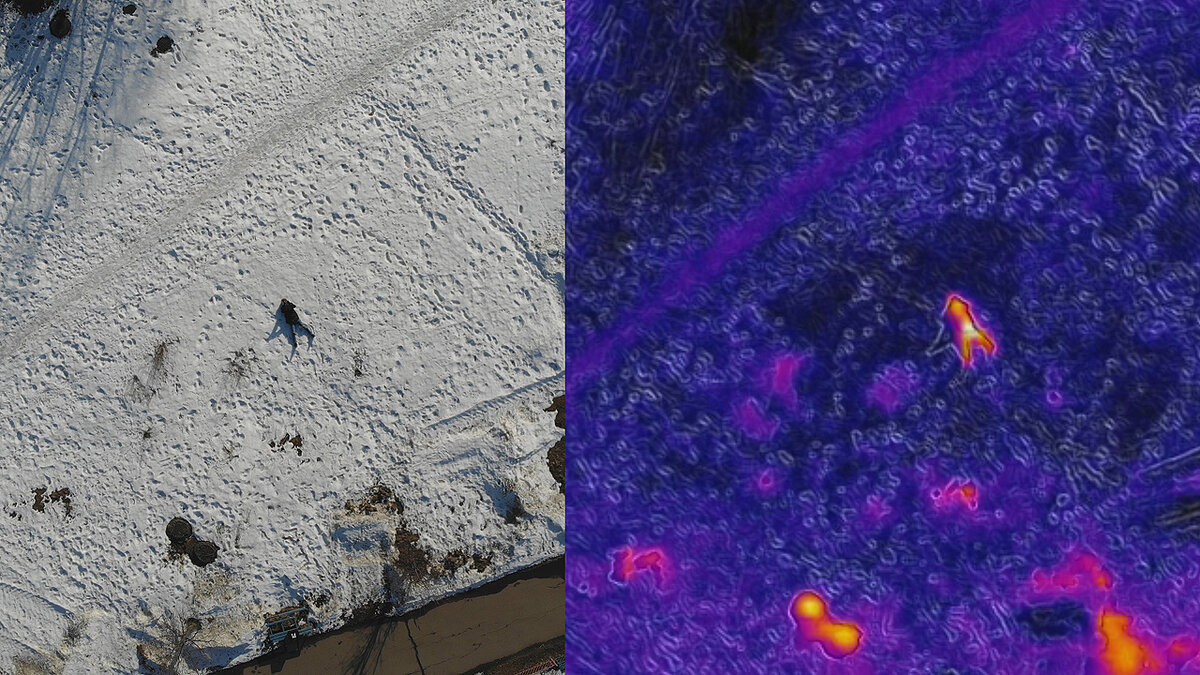
\includegraphics[width=0.8\linewidth]{my_folder/images/teplovision.jpeg}
    \caption{Пример съемки на Mavic 2 Enterprise Dual с высоты 40 метров}
    \label{teplovision}
\end{figure}

Телевизионные камеры имеют существенный недостаток: погодные условия, такие как дождь, снег и туман, затрудняют видимость или делают её невозможной. Проблему видимости в экстремальных условиях можно решить с помощью тепловизоров. Однако тепловизоры также имеют недостатки. Из-за низкой пространственной разрешающей способности они не показывают мелкие детали наблюдаемой сцены. Кроме того, тепловизоры эффективны только для объектов с температурой, отличающейся от температуры окружающей среды, то есть при наличии температурного контраста.

Полезными признаками для телевизионных изображений являются \cite{optical-prisnaki}:
\begin{itemize}
    \item форма,
    \item размеры,
    \item текстура,
    \item внутренняя структура объектов,
    \item окружение.
\end{itemize}

Полезными признаками для тепловизионных изображений являются:
\begin{itemize}
    \item форма,
    \item  максимальное/минимальное значение эмиссии,
    \item  количество и расположение горячих пятен,
    \item окружение (среда). 
\end{itemize}

Распознавание трехмерных объектов по их двумерным изображениям стало одной из ключевых задач анализа сцен и компьютерного зрения. Объектом считается не только цифровое представление фрагмента двумерной сцены, но и его приближенное описание в виде набора характерных свойств (признаков). Признаки – это измерения, используемые для классификации объектов \cite{rasposnavanie}.

При реализации задачи локализации решение может формулироваться следующим образом: на основе априорной информации о рассматриваемой сцене (участке земной поверхности) и апостериорной информации, полученной в процессе полета, сопоставляются текущее и эталонное изображения. Это позволяет локализовать заданные объекты сцены на текущем изображении и определить их текущие координаты для формирования управляющих сигналов для беспилотного летательного аппарата \cite{insarov}.

\section{Анализ методов машинного обучения}
\subsection{Сверточные нейронные сети}
Сверточные нейронные сети представляют собой класс искусственных нейронных сетей, специально разработанных для обработки и анализа изображений. Их архитектура и механизмы позволяют эффективно распознавать сложные паттерны в визуальных данных, что делает их незаменимыми в различных областях компьютерного зрения \cite{Krizhevsky2012ImageNetCW}.

Основными компонентами являются сверточные слои, слои объединения (пулинга) и полностью связанные слои.
\begin{enumerate}[1.]
    \item Сверточные слои выполняют операцию свертки, применяя фильтры или ядра к исходному изображению. Фильтры помогают выделять различные признаки, такие как края, углы и текстуры. Каждый фильтр генерирует карту признаков, которая подчеркивает определенные аспекты входного изображения.
    \item Слои объединения пулинга уменьшают размерность карт признаков, что снижает вычислительную нагрузку и вероятность переобучения. Наиболее распространенными методами объединения являются максимальный пулинг (максимальное значение в каждом подокне) и средний пулинг (среднее значение в каждом подокне).
    \item Полностью связанные слои находятся в конце сети и служат для окончательной классификации. Они соединяют все нейроны предыдущего слоя с каждым нейроном текущего слоя, позволяя учитывать все выделенные ранее признаки.
\end{enumerate}

Сверточные нейронные сети обладают рядом преимуществ, делающих их эффективными для обработки изображений. В первую очередь свойства сверточных слоев позволяют учитывать локальные пространственные отношения между пикселями, что важно для распознавания объектов. Использование методов, таких как нормализация локальных откликов и Dropout, помогает уменьшить вероятность переобучения. Также, сверточные нейронные сети могут эффективно обучаться на больших объемах данных благодаря использованию графических процессоров (\textit{GPU}), что значительно ускоряет процесс обучения.

Сверточные нейронные сети широко применяются для решения различных задач в области классификации изображений. Например, используются для идентификации и верификации лиц на изображениях и в видео; помогают в анализе медицинских изображений, таких как рентгеновские снимки и МРТ, для обнаружения патологий; используются для распознавания объектов и ситуаций на дорогах, что необходимо для безопасного управления транспортом.

Современные исследования в области сверточных нейронных сетей направлены на улучшение архитектуры и алгоритмов обучения. Разрабатываются новые методы нормализации и регуляризации, такие как \textit{Batch Normalization} и новые типы нелинейностей (например, \textit{ReLU}). Ведутся работы по созданию более эффективных моделей, которые требуют меньше вычислительных ресурсов и могут работать в реальном времени.

\subsection{\textit{Aggregate Channel Features}}
Метод \textit{ACF (Aggregate Channel Features)} является инновационным подходом в области распознавания лиц, который направлен на решение проблем, связанных с большими изменениями внешнего вида лиц в естественных условиях. Данный метод опирается на концепцию каналов изображения, расширяя их до различных типов, таких как градиенты и гистограммы ориентированных градиентов, что позволяет кодировать разнообразную признаками информацию в простой форме \cite{ACF}.

Исторически, одним из самых влиятельных подходов к распознаванию лиц был метод \textit{Viola-Jones}, который использует прямоугольные признаки, похожие на признаки Хаара, и обучает классификатор с помощью алгоритма \textit{Adaboost}. Этот метод достиг значительных успехов в распознавании лиц в реальном времени, но его производительность все еще оставалась ограниченной из-за большой изменчивости внешнего вида лиц в неконтролируемых условиях. Для преодоления этого ограничения метод \textit{ACF} использует расширенные каналы изображения, такие как градиенты и гистограммы ориентированных градиентов, что позволяет более эффективно кодировать информацию о лицах.

Метод \textit{ACF} включает в себя несколько ключевых аспектов. Во-первых, он использует расширенные каналы изображения для кодирования разнообразной информации. Например, цветовые каналы в пространстве \textit{LUV}, каналы градиентной величины и гистограммы градиентов в \textit{RGB} пространстве показывают наилучшие результаты при распознавании лиц. Эти каналы обеспечивают богатую репрезентационную способность, что особенно важно для обработки лиц с различными выражениями и позами.

Во-вторых, метод \textit{ACF} предусматривает мультискейлинг представления признаков, что позволяет еще больше обогатить репрезентацию. В оригинальной версии метода все признаки имели одинаковый масштаб, но эксперименты показали, что мультискейлинг улучшает производительность. Это достигается за счет изменения масштаба восприятия, локального масштаба и масштаба интеграции признаков.

Третьим важным аспектом является подход к мультивидовому распознаванию лиц, который использует повторную ранжировку оценок и корректировку обнаружений. Это помогает эффективно справляться с различными позами лиц и улучшает точность локализации лиц в изображениях. В результате, метод \textit{ACF} демонстрирует конкурентоспособные результаты на сложных наборах данных, таких как \textit{AFW} и \textit{FDDB}, показывая высокую точность и скорость распознавания (до 42 кадров в секунду на изображениях \textit{VGA}).

Метод \textit{ACF} значительно улучшает производительность распознавания лиц благодаря тщательному исследованию и оптимизации различных параметров признаков. Он предлагает более быструю и точную альтернативу традиционным методам распознавания лиц, обеспечивая богатую репрезентацию и высокую эффективность вычислений.

\subsection{\textit{Deformable Part Models}}
Метод деформируемых частей (\textit{Deformable Part Models, DPM}) представляет собой один из эффективных подходов к обнаружению объектов на изображениях. Этот метод был разработан для улучшения точности и эффективности поиска объектов, особенно в условиях сложного фона и объектов в различных позах \cite{DPM}. 

Основная идея метода \textit{DPM} заключается в моделировании объектов как совокупности частей, которые могут деформироваться относительно друг друга. Каждая часть описывается своим собственной подмоделью, которая оценивает вероятность нахождения этой части объекта в определённом месте изображения. Главным преимуществом такого подхода является возможность учёта различных положений и деформаций частей объекта, что значительно улучшает результаты обнаружения по сравнению с более простыми моделями машинного обучения.

Основой метода \textit{DPM} является использование каскадных классификаторов. В данном контексте каскадный классификатор представляет собой последовательность всё более сложных моделей, которые последовательно отсекают маловероятные гипотезы обнаружения объектов. Сначала применяется простая модель, которая быстро отбрасывает большую часть областей изображения. Затем, на оставшихся областях, применяются более сложные модели, которые более точно определяют положение и конфигурацию частей объекта.

Для реализации \textit{DPM} с каскадными классификаторами используется несколько ключевых компонент.
\begin{enumerate}[1.]
    \item Использование моделей звездной структуры, в которых все части объекта привязаны к одной "корневой" части, упрощает вычисления и позволяет эффективно использовать динамическое программирование для поиска оптимальных конфигураций частей.
    \item На ранних этапах каскада используются упрощённые модели частей, которые быстрее вычисляются. Это позволяет быстро отсеивать маловероятные гипотезы без значительных затрат вычислительных ресурсов.
    \item Методы динамического программирования и обобщённого дистанционного преобразования позволяют эффективно учитывать зависимости между частями объекта. Вместо того чтобы рассматривать каждую часть отдельно, используются общие характеристики и взаимосвязи, что значительно ускоряет процесс обнаружения.
    \item Для отсеивания гипотез на каждом этапе каскада используются вероятностно допустимые пороги (\textit{PAA thresholds}). Они выбираются на основе статистики частичных гипотез по положительным примерам и гарантируют, что с высокой вероятностью не будут отсеяны гипотезы, ведущие к правильным обнаружениям.
\end{enumerate}

Данный метод показывает высокую эффективность на различных наборах данных, таких как \textit{PASCAL VOC}, демонстрируя способность точно обнаруживать объекты в условиях разнообразных поз, масштабов и фонов. 

Метод \textit{DPM} обладает рядом преимуществ, включая гибкость и способность учитывать сложные деформации объектов, что делает его эффективным инструментом для задач обнаружения объектов в условиях реального мира. Однако, несмотря на свою эффективность, метод требует значительных вычислительных ресурсов, что может ограничивать его использование в некоторых задачах. 

\subsection{Случайный лес}
Случайный лес (\textit{Random Forest}) — метод ансамблевого обучения, используемый для задач классификации и регрессии. Состоит из множества независимых деревьев решений, которые работают совместно для повышения точности прогноза и уменьшения вероятности переобучения \cite{random-forest}.

Алгоритм Случайного леса был впервые предложен в 1995 году Тин Кам Хо и позднее расширен Лео Брейманом и Адель Катлер. Основной принцип метода заключается в объединении большого числа деревьев решений, обученных на различных подмножествах данных и случайных подмножествах признаков, чтобы обеспечить более стабильные и надежные предсказания. В случае задач классификации итоговый результат определяется большинством голосов деревьев, а в задачах регрессии — средним значением их предсказаний.

Одним из ключевых преимуществ Случайного леса является его устойчивость к переобучению. Это достигается за счет использования метода \textit{bagging} (\textit{bootstrap aggregating}), при котором для каждого дерева выбирается случайная подвыборка данных с возвращением, что создает множество различных обучающих наборов. Каждый из этих наборов используется для обучения отдельного дерева, а затем результаты их предсказаний объединяются. Добавление случайности на этапе выбора признаков при построении деревьев также снижает корреляцию между деревьями и способствует уменьшению переобучения.

Среди других преимуществ Случайного леса можно отметить:
\begin{itemize}
    \item благодаря объединению множества деревьев, метод обеспечивает высокую точность предсказаний;
    \item может применяться как для задач классификации, так и для регрессии;
    \item позволяет легко определить, какие признаки оказывают наибольшее влияние на предсказание, используя такие метрики, например, как \textit{Gini importance} и \textit{mean decrease in impurity (MDI)};
    \item  эффективно справляется с пропущенными данными, сохраняя высокую точность предсказаний.
\end{itemize}

Однако, у метода есть и свои недостатки. Он может быть ресурсоемким и требовать значительных вычислительных мощностей и времени на обучение, особенно при работе с большими наборами данных. Кроме того, интерпретируемость модели Случайного леса ниже по сравнению с отдельными деревьями решений, что может затруднить объяснение полученных результатов.

\subsection{Сравнительный анализ}
В таблице \ref{tab:ml-compare} представлено сравнение методов машинного обучения для решения задачи обнаружения объектов на изображении. Рассмотрены преимущества и недостатки таких методов, как Сверточные нейронные сети, Aggregate Channel Features, Deformable Parts Models, Случайный лес.
\begin{longtable}{|l|l|l|l|}
\caption{Сравнение методов машинного обучения}
\label{tab:ml-compare}\\
\hline
\multicolumn{1}{|c|}{Метод}                                                                                                    & \multicolumn{1}{c|}{Описание}                                                                                                                                                                                                         & \multicolumn{1}{c|}{Преимущества}                                                                                                                                                                                                                                              & \multicolumn{1}{c|}{Недостатки}                                                                                                                                                                               \\ \hline
\endhead
%
\textit{\begin{tabular}[c]{@{}l@{}}Convolutional \\ Neural \\ Network \\ (CNN)\\ Сверточные \\ нейронные \\ сети\end{tabular}} & \begin{tabular}[c]{@{}l@{}}Глубокая \\ нейронная сеть, \\ использующая \\ сверточные слои \\ для автомати-\\ ческого извлечения \\ признаков из \\ изображений.\end{tabular}                                                          & \begin{tabular}[c]{@{}l@{}}Высокая \\ точность \\ распознавания, \\ автоматическое \\ извлечение \\ признаков, \\ устойчивость \\ к деформации \\ распознаваемых \\ изображений.\end{tabular}                                                                                  & \begin{tabular}[c]{@{}l@{}}Необходимо \\ большое количество \\ размеченных данных \\ для обучения, \\ требуются большие \\ вычислительные \\ ресурсы  \\ (GPU).\end{tabular}                                  \\ \hline
\textit{\begin{tabular}[c]{@{}l@{}}Aggregate \\ Channel \\ Features \\ (ACF)\end{tabular}}                                     & \begin{tabular}[c]{@{}l@{}}Метод, который \\ извлекает признаки \\ из нескольких \\ каналов \\ изображения \\ (например, оттенки \\ серого, RGB) и \\ агрегирует их \\ для обнаружения \\ объектов.\end{tabular}                      & \begin{tabular}[c]{@{}l@{}}Подходит для \\ работы в \\ реальном \\ времени, \\ хорошо \\ работает \\ с небольшим \\ количеством \\ данных, \\ высокая \\ точность \\ локализации\\ объектов на \\ изображениях \\ при\\ использовании\\ совместно с \\ бустингом.\end{tabular} & \begin{tabular}[c]{@{}l@{}}Более низкая \\ точность по \\ сравнению с \\ методами глубокого \\ обучения, ограничен \\ простыми \\ признаками, не \\ подходит для \\ сложных сцен.\end{tabular}                \\ \hline
\textit{\begin{tabular}[c]{@{}l@{}}Deformable \\ Parts Models\\ (DPM)\end{tabular}}                                            & \begin{tabular}[c]{@{}l@{}}Использует \\ графическую \\ модель частей \\ объекта \\ (неориентирован-\\ ный граф) и их \\ пространственные \\ отношения для \\ обнаружения и \\ локализации \\ объектов.\end{tabular}                  & \begin{tabular}[c]{@{}l@{}}Может \\ моделировать \\ деформации \\ объектов, \\ хорошо \\ работает \\ с представле-\\ нием объектов \\ на основе \\ частей.\end{tabular}                                                                                                        & \begin{tabular}[c]{@{}l@{}}Вычислительно \\ затратен, может \\ быть медленнее, \\ чем CNN, \\ производительность \\ сильно зависит от \\ качества моделей \\ частей.\end{tabular}                             \\ \hline
\textit{\begin{tabular}[c]{@{}l@{}}Random \\ Forest\\ Случайный \\ лес\end{tabular}}                                           & \begin{tabular}[c]{@{}l@{}}Метод ансамблевого \\ обучения, в ходе\\ которого строится\\ большое количество \\ деревьев решений, \\ а результатом \\ классификации \\ является наиболее\\ часто \\ встречающийся\\ класс.\end{tabular} & \begin{tabular}[c]{@{}l@{}}Устойчив к \\ переобучению, \\ хорошая \\ производитель-\\ ность при \\ ограниченных \\ вычислительных \\ ресурсах, может \\ обрабатывать \\ различные \\ типы данных.\end{tabular}                                                                 & \begin{tabular}[c]{@{}l@{}}Более низкая \\ точность по \\ сравнению с \\ методами \\ глубокого обучения, \\ требует \\ тщательного \\ выбора признаков, \\ может быть \\ чувствителен \\ к шуму.\end{tabular} \\ \hline
\end{longtable}
Сверточные нейронные сети обеспечивают высокую точность и могут обрабатывать сложные сцены, но требуют больших вычислительных ресурсов и больших наборов данных для обучения. Метод \textit{ACF} эффективен и быстр, подходит для работы в реальном времени, но имеет меньшую точность в сложных сценах. Метод \textit{DPM} хорошо справляется с моделированием деформаций объектов, однако он вычислительно затратен. Случайный лес устойчив к переобучению и работает с ограниченными ресурсами, но может быть менее точным по сравнению с методами глубокого обучения. 

\section{Анализ классических алгоритмов}
\subsection{Вычитание фона}
Метод вычитания фона (\textit{background subtraction}) является популярным подходом для выделения движущихся объектов на видео, снятом стационарной камерой. Он служит первым шагом в многоступенчатых системах компьютерного зрения, которые решают задачи мониторинга, распознавания и отслеживания объектов. Основная задача этого метода заключается в том, чтобы на каждом кадре видео отличать пиксели, принадлежащие движущимся объектам, от пикселей фона. Это достигается путем сравнения текущего кадра с моделью фона, которая представляет собой статическое изображение сцены без движущихся объектов.

Основное уравнение вычитания фона можно представить следующим образом:
\[ M_t(s) = \begin{cases} 
1, & \text{если} \, d(C_t(s), B_t(s)) > \theta \\
0, & \text{иначе}
\end{cases} \]
где \( M_t(s) \) — метка движения в момент времени \( t \) для пикселя \( s \), \( B_t(s) \) — модель фона для пикселя \( s \) в момент времени \( t \), \( C_t(s) \) — цвет пикселя \( s \) в момент времени \( t \), \( d \) — метрика расстояния между цветом пикселя и моделью фона, \( \theta \) — пороговое значение.

Методы вычитания фона можно классифицировать на две основные группы: методы, основанные на временных различиях между последовательными изображениями, и методы, использующие сравнение текущего изображения с заранее подготовленными моделями фона. Рассмотрим три наиболее распространенных метода: метод интеркадровых различий, метод приблизительного медианного фильтра и модель гауссовых смесей (\textit{GMM}).

Метод интеркадровых различий использует разницу между последовательными кадрами для выделения движущихся объектов. Его основное преимущество заключается в быстроте выполнения, однако он чувствителен к изменениям освещения и подвержен эффекту "камуфляжа"{}, когда объект сливается с фоном по цвету. Обновление модели фона в этом методе можно описать формулой:
\[ B_{t+1}(s) = (1 - \alpha) B_t(s) + \alpha C_t(s) \]
где \( \alpha \) — константа, определяющая скорость обновления модели фона.

Метод приблизительного медианного фильтра предлагает более устойчивую к шуму модель фона, обновляя её путем медианной фильтрации нескольких последовательных кадров. Этот метод лучше справляется с динамическими изменениями фона, однако требует большего объема вычислений и памяти.

Модель гауссовых смесей (\textit{GMM}) представляет фон как набор гауссовых распределений, что позволяет эффективно справляться с изменениями освещения и динамическими фонами. Несмотря на высокую точность, этот метод требует значительных вычислительных ресурсов и памяти, что делает его менее пригодным для применения в системах с ограниченными ресурсами, таких как встраиваемые системы и \textit{IP}-камеры.

Эффективность рассмотренных методов может оцениваться по таким параметрам, как время вычислений, потребление памяти и точность (\textit{precision/recall}). Результаты исследований \cite{Brutzer2011EvaluationOB} показывают, что методы интеркадровых различий и приблизительного медианного фильтра значительно быстрее и требуют меньше памяти по сравнению с \textit{GMM}. Однако \textit{GMM} обеспечивает более высокую точность за счет учета сложных изменений фона и освещения.
\subsection{Оптический поток}
Метод оптического потока является важным инструментом в компьютерном зрении, предназначенным для оценки движения объектов в последовательности изображений. Он основывается на предположении о сохранении яркости: интенсивность пикселей переносится из одного кадра в следующий без изменений\cite{fleet}. Основное уравнение, используемое в данном методе, выглядит следующим образом:
\[ I(\mathbf{x}, t) = I(\mathbf{x} + \mathbf{u}, t + 1) \]
где \( I(\mathbf{x}, t) \) — интенсивность изображения в точке \(\mathbf{x}\) в момент времени \( t \), а \(\mathbf{u} = (u_1, u_2)^T \) — двумерная скорость.

Основным подходом к оценке оптического потока является градиентный метод. Он предполагает, что изменения интенсивности во времени малы, что позволяет использовать линейную аппроксимацию:
\[ I_t + \nabla I \cdot \mathbf{u} = 0 \]
где \( I_t \) — временная производная интенсивности, а \(\nabla I\) — пространственные производные. Для решения этого уравнения используется метод наименьших квадратов, минимизирующий функцию ошибки:
\[ E(\mathbf{u}) = \sum_k w_k (\nabla I(\mathbf{x}_k) \cdot \mathbf{u} + I_t(\mathbf{x}_k))^2 \]
где \( w_k \) — весовые коэффициенты, определяющие вклад каждого пикселя в общую ошибку.

Однако, при использовании этого метода возникают проблемы с неоднозначностью решений, особенно в областях с низкой текстурой. Для преодоления этой проблемы применяются итеративные методы, такие как метод Гаусса-Ньютона, которые уточняют оценку оптического потока за несколько шагов, уменьшая остаточную ошибку.

Одной из важных задач при оценке оптического потока является обработка границ объектов и областей с разными движениями. Для этого используются модели смешивания, которые предполагают наличие нескольких движущихся объектов и учитывают вероятность принадлежности каждого пикселя к той или иной модели движения. Формула функции ошибки для смеси моделей выглядит следующим образом:
\[ E(\mathbf{u}_n) = \sum_k q_n(\mathbf{x}_k) [\nabla I(\mathbf{x}_k, t) \cdot \mathbf{u}_n + I_t(\mathbf{x}_k, t)]^2 \]
где \( q_n(\mathbf{x}_k) \) — вероятность того, что пиксель \(\mathbf{x}_k\) принадлежит модели движения \(\mathbf{u}_n\).

Для улучшения точности оценки оптического потока используются многомасштабные представления изображений, которые позволяют избежать локальных минимумов, и устойчивые функции стоимости, способные обрабатывать выбросы. Дополнительно согут использоваться фазовые методы, которые основываются на разложении изображения на полосовые каналы и предполагают сохранение фазы в каждом канале:
\[ \nabla \phi(\mathbf{x}, t) \cdot \mathbf{u} + \phi_t(\mathbf{x}, t) = 0 \]
где \(\phi(\mathbf{x}, t)\) — фаза комплексного полосового сигнала \( r(\mathbf{x}, t) \).

Метод оптического потока является мощным инструментом для анализа движения, однако требует дальнейших исследований для улучшения учета изменений яркости в длительных последовательностях изображений.
\subsection{Сравнительный анализ}
Проведем сравнение классических алгоритмов обнаружения объектов на изображениях или в видеопотоке (таблица \ref{tab:classical-methods}).
\begin{longtable}{|l|l|l|l|}
\caption{Сравнение классических алгоритмов}
\label{tab:classical-methods}\\
\hline
\multicolumn{1}{|c|}{Метод}                                & \multicolumn{1}{c|}{Описание}                                                                                                                                        & \multicolumn{1}{c|}{Преимущества}                                                                                                                                  & \multicolumn{1}{c|}{Недостатки}                                                                                                                                                              \\ \hline
\endhead
%
\begin{tabular}[c]{@{}l@{}}Вычитание \\ фона\end{tabular}  & \begin{tabular}[c]{@{}l@{}}Обнаруживает \\ движущиеся \\ объекты путем \\ вычитания \\ текущего кадра \\ из эталонной \\ модели фона.\end{tabular}                   & \begin{tabular}[c]{@{}l@{}}Простой, быстрый \\ и вычислительно \\ эффективный, \\ хорошо подходит \\ для статических \\ настроек камеры.\end{tabular}              & \begin{tabular}[c]{@{}l@{}}Проблемы с \\ динамическим \\ фоном, \\ изменениями \\ освещения и \\ сложными \\ сценами, \\ неустойчив \\ к движению \\ камеры.\end{tabular}                    \\ \hline
\begin{tabular}[c]{@{}l@{}}Оптический\\ поток\end{tabular} & \begin{tabular}[c]{@{}l@{}}Вычисляет \\ движение \\ объектов между \\ последовательными \\ кадрами на основе \\ изменений \\ интенсивности \\ пикселей.\end{tabular} & \begin{tabular}[c]{@{}l@{}}Может захватывать \\ информацию о \\ движении, полезен \\ для обнаружения \\ движущихся \\ объектов \\ независимо от фона.\end{tabular} & \begin{tabular}[c]{@{}l@{}}Вычислительно \\ затратен, \\ чувствителен \\ к шуму и \\ быстрым \\ движениям, \\ может иметь \\ проблемы со \\ сложными \\ принципами \\ движения.\end{tabular} \\ \hline
\end{longtable}
Наилучшие результаты могут быть достигнуты при использовании гибридных подходов. Например, при комбинации сверточных нейронных сетей с алгоритмом оптического потока можно объединить преимущества глубокого обучения для точной классификации и оптического потока для детекции движения. Такой подход позволяет улучшить точность и надежность системы, справляясь как с детекцией сложных объектов, так и с анализом движения в динамичных сценах. Впервые данный подход был представлен в статье \cite{cof} как алгоритм под названием <<С-FO>>. 

Внедрение гибридных методов позволяет учитывать сильные стороны каждого из алгоритмов, минимизируя их недостатки. Это особенно важно в условиях реального времени, где требуется высокая производительность и точность при ограниченных вычислительных ресурсах.

\section{Разработка гибридного алгоритма}
\subsection{Математическая постановка задачи}
Для постановки задачи обнаружения введем стохастический процесс $Y(t)$:

\begin{equation}
Y(t) = \{Y_t \mid M \times A \times I, t \},
\end{equation}

где:
\begin{itemize}
    \item \( Y_t \) — набор параметров, описывающий позицию обнаруживаемого объекта, в данном случае ограничивающий прямоугольник в измерении изображения с вложенным в него участком этого изображения, в комбинированном пространстве,
    \item \( M \) — пространство признаков движения,
    \item \( A \) — пространство признаков внешнего вида,
    \item \( I \) — пространство признаков инфракрасного излучения,
    \item \( t \) - дискретный временной шаг.
\end{itemize}
 
Несмотря на то, что точное математическое описание движения и изображения объекта возможно, в большинстве случаев оно является вычислительно трудноразрешимым, потому процесс является стохастическим.

 Функция $\tau$ осущствляет отображение признаков объекта в пространство его положений \textit{Y}
\begin{equation}
\tau : \textbf{N} \rightarrow M \times A \times I, t \rightarrow \tau(t).
\end{equation}

В рассматриваемой нами задаче $\tau$ формируется как сложная функция:
\begin{equation}
\label{tau_t}
\tau(t) = \delta(X(t)),
\end{equation}

где $X(t)$ – последовательность изображений из пространства $L_c$:
\begin{equation}
X(t) = \{X_t \in L_c, t \in \textbf{N}\},
\end{equation}

обрабатываемая функцией:
\begin{equation}
\delta : L_c \rightarrow M \times A \times I, X(t) \rightarrow \delta(X(t)).
\end{equation}

С учетом измерений, учитываемых функцией $\tau$, уравнение (\ref{tau_t}) представим в следующем виде:
\begin{equation}
\label{tau_t_advanced}
\tau(t) = \delta(X(t), Y(t - 1)).
\end{equation}

Использование уравнения (\ref{tau_t_advanced}) предполагает значительное использование вычислительных ресурсов, поэтому на практике вводится ограничивающий параметр $n$:
\begin{equation}
\tau(t) = \delta(X(t) \setminus X(t - n), Y(t - 1) \setminus Y(t - n)).
\end{equation}

Суть данной работы заключается в поиске оператора $\delta$, который является алгоритмом обнаружения объектов.
\subsection{Обзор гибридного алгоритма}
Основная задача, которую необходимо решить при обнаружении движущихся объектов с борта беспилотного летательного аппарата (БПЛА), заключается в необходимости различать изменения в кадре, вызванные движением БПЛА, от изменений, вызванных движущимися объектами. Для этого проводится первый этап предобработки изображений, в ходе которого извлекаются особые точки. На следующем этапе происходит классификация объектов с использованием гибридного классификатора.
\subsection{Оценка параметров движения}
Блок-схема алгоритма оценки параметров движения представлена на рис. \ref{fig:dvizh}. Задача данного алгоритма заключается в предобработке получаемых кадрах, а именно, в формировании переченя потенциальных объектов, которые имеют перемещение во времени. Для этого производится двухэтапная оценка на соответствие фона в текущем и предыдущем кадрах видеопотока: расчет глобальной модели движения на каждом изображении, а затем выравнивание за счет модели движения. Таким образом, разница моделей движения двух последовательных изображений дает представление о подвижных объектах, имеющих непостоянное и отличающееся от фонового изменение параметров движения, что дает возможность детально изучать полученные области на предмет поиска искомых объектов путем формирования особых точек.

Алгоритм оценки движения реализована в пять этапов: выбор точек привязки, локальная оценка движения, глобальная оценка движения, вычитание фона, извлечение особых точек.
  \begin{figure}[ht!]
    \centering
    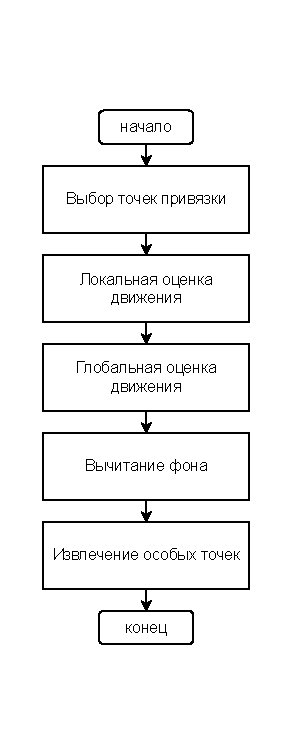
\includegraphics[width=0.3\linewidth]{my_folder/images/движение.pdf}
    \caption{Блок-схема алгоритма оценки параметров движения}
    \label{fig:dvizh}
\end{figure}

\textbf{Выбор точек привязки}

Для выбора точек привязки используется метод \textit{Good Features to Track}, который был предложен Карло Томази и Джианбо Ши в 1994 году \cite{goodTruck}. Данный метод направлен на выявление таких характеристик в изображениях, которые могут быть надежно отслежены в последовательных кадрах.

Метод основывается на анализе малых матриц автокорреляции изображения. Рассматривается 2x2 матрица \( Z \), элементы которой зависят от градиентов интенсивности изображения в окне размером \( W \times W \). Формула для элементов матрицы \( Z \):
   \begin{equation}
   Z = \sum_{x, y \in W} \begin{bmatrix} I_x^2 & I_x I_y \\ I_x I_y & I_y^2 \end{bmatrix}
   \end{equation}
   где \( I_x \) и \( I_y \) — градиенты интенсивности изображения по осям \( x \) и \( y \) соответственно.

Хорошие характеристики должны удовлетворять двум условиям:
\begin{itemize}
\item значения собственных чисел матрицы \( Z \) должны быть достаточно большими, чтобы преодолеть уровень шума изображения;
\item собственные числа не должны сильно отличаться по величине, что обеспечивает хорошую обусловленность матрицы.
\end{itemize}

Если собственные числа \( \lambda_1 \) и \( \lambda_2 \) матрицы \( Z \) велики и примерно равны, то окно содержит текстуру, которая хорошо отслеживается. В противном случае, окно либо содержит однородную область (оба собственных числа малы), либо одно из собственных чисел значительно меньше другого (одномерный паттерн).

\textbf{Локальная оценка движения}

Извлеченные из предыдущего кадра точки привязки алгоритму оптического потока Лукаса-Канаде с пирамидальной структурой \cite{Bouguet1999PyramidalIO}. Цель алгоритма состоит в отслеживании точки \( u \) на кадре \( I_k \) (где \( k \) - номер кадра) и её перемещении в другое местоположение \( v \) на кадре \( I_{k+1} \). Разница между точками \( u \) и \( v \) представляет собой вектор оптического потока для этой точки, который описывает как угол движения, так и величину, с которой точка \( u \) перемещается с кадра \( I_k \) на \( v \) кадр \( I_{k+1} \). Этот процесс применяется ко всем ключевым точкам, извлечённым из предыдущего кадра изображения, для определения их соответствующих положений на текущем кадре изображения.

\textbf{Глобальная оценка движения}

После вычисления векторов смещения оптического потока они нормализуются и объединяются с помощью алгоритма кластеризации \textit{ELM} \cite{ELM}. Координаты \( x \) и \( y \) векторов оптического потока, которые охватывают как угол движения, так и смещение оптического потока, используются в качестве признаков для кластеризации. Метод \textit{Evolving Local Means} работает за один проход, рекурсивно вычисляя локальное среднее и дисперсию кластеров.

Кластер с наибольшим количеством векторов оптического потока, связанных с ним, представляет движение камеры относительно фона. Признаки, содержащиеся в самом большом кластере, который отражает движение камеры, затем используются для вычисления матрицы гомографии с использованием алгоритма случайной выборки для улучшения устойчивости и удаления оставшихся выбросов. Выбор \textit{ELM} вместо альтернатив, таких как алгоритм сдвига среднего значения, был обусловлен его вычислительной эффективностью, причем оба подхода обеспечивают сопоставимую точность. 

Введение небольших ошибок \textit{ELM} минимизируется при помощи алгоритма случайной выборки консенсуса (\textit{RANSAC}) при вычислении гомографии. Минимальный размер объекта ограничивается процессом кластеризации, удаляются кластеры размером менее 10 пикселей для подавления шума. Если движущийся объект останавливается на продолжительный период времени, подход перестает его обнаруживать, так как \textit{RDE} является детектором на основе движения. Чистое вращение представляет сложность для предложенного подхода из-за использования оптического потока при вычислении матрицы гомографии.

\textbf{Вычитание фона}

На этом этапе происходит вычитание движущегося фона, чтобы выделить области, в которых не произошли изменения. Это необходимо из-за того, что параметры движения движущихся объектов отличаются от модели движения фона.

Для того чтобы вычислить изображение фона, оценивается предыдущий кадр:
\begin{equation}
\overbrace{X_{n-1}}^n(s)=X_n\left(T\left(H_n, s\right)\right),
\end{equation}
где $\overbrace{n-1}(s)$ - оценка предыдущего кадра, $s$ координаты точки. Затем вычитаемое изображение фона $E_{n-1}$ для $X_{n-1}$ вычисляется как:
\begin{equation}
E_{n-1}=|X_{n-1}-\overbrace{n-1}| \text {. }
\end{equation}

\textbf{Извлечение особых точек}

На этом этапе определяются точки фона вычитаемого изображения и извлекаются области на исходном изображении и фоне вычитаемого изображении, расположенного вокруг особых точек. Вычитая расчетный фон, движущиеся объекты остаются заметными на вычитаемом изображении. Таким образом определяется местоположение областей, определяющих выделенную точку на вычитаемом фоне изображения.

\subsection{Гибридный классификатор}

\textbf{Классификатор внешнего вида}

Архитектура нейронной сети классификатора внешнего вида состоит из 16 фильтров с размером сверточных ядер 3х3, после которых применяется функция активации ReLU, затем из 32 фильтров с размером ядер 3х3, активацией ReLU и операцией объединения (pooling). Аналогично применяется еще 64 фильтра. В конце сети идет полносвязный слой с функцией активации softmax, где для каждой особой точки $q_{n, i}$ получаем вероятность принадлежности к классу $p_{n, i}^a$.

Также после каждой функции активации были использованы исключающие слои (dropout) и пакетная нормализация для регуляризации процесса обучения.

\textbf{Классификатор движения}

Разница в движении $d_{n, i}$ для движущегося объекта при $q_{n-1, i}$ между перспективным и локальным движением определяется следующим образом:
$$
d_{n, i}=T\left(H_n, q_{n-1, i}\right)-\tilde{q_{n, i}} .
$$

где $\tilde{q_{n, i}}$ - соответствующая точка в текущем кадре, полученная с помощью оценки параметров локального движения особых точек с помощью согласования оптического потока Лукаса - Канаде, $v_{n, i}$ - обратное локальное движение, которое можно вычислить с помощью уравнения 
\begin{equation}
v_{n, i}=\arg \min _u \sum_{s \in N\left(\widetilde{p_{n, i}}\right)}\left|X_n(s)-X_{n-1}(s-u)\right|^2,
\end{equation}

Кроме того, были введены следующие характеристики: $u_{n, i}=\tilde{q_{n, i}}-q_{n-1, i}$ и $h_{n, i}=T\left(H_n, q_{n-1, i}\right)-q_{n-1, i}$. Эта разница в движении представляет собой фактическую скорость движущегося объекта по отношению к параметрам движения фона.

Таким образом, можно ввести параметры движения, которые описывают характер движения объекта в оптическом потоке. Данные параметры приведены в таблице \ref{tab:moving}.

\begin{table}[ht!]
\centering
\begin{tabular}{|c|c|c|}
\hline
№  & Параметр                                                                         & Описание                                                                                     \\ \hline
1. & $l_{n, i}=\left\|d_{n, i}\right\|_2$                                             & \begin{tabular}[c]{@{}c@{}}Величина разности \\ движений\end{tabular}                        \\ \hline
2. & $\alpha_{n, i}=\arctan \left(d_{n, i}\right)$                                    & \begin{tabular}[c]{@{}c@{}}Угол разности \\ движений\end{tabular}                            \\ \hline
3. & $\epsilon_{n, i}=\left\|u_{n, i}-v_{n, i}\right\|_2$                             & \begin{tabular}[c]{@{}c@{}}Двунаправленное \\ контрольное расстояние\end{tabular}            \\ \hline
4. & $\theta_{n, i}=\arctan \left(h_{n, i}\right)-\arctan \left(u_{n, i}\right)$      & \begin{tabular}[c]{@{}c@{}}Перспективно-локальная \\ разница углов движения\end{tabular}     \\ \hline
5. & $\delta_{n, i}=\left|\left\|h_{n, i}\right\|_2-\left\|u_{n, i}\right\|_2\right|$ & \begin{tabular}[c]{@{}c@{}}Перспективно-локальная \\ разница амплитуды движения\end{tabular} \\ \hline
\end{tabular}
    \caption{Значения параметров движения объекта}
    \label{tab:moving}
\end{table}

После составления из данных значений вектор-признаков был обучен классификатор селекции ложных объектов, основанный на полносвязной нейронной сети. Структурная схема архитектуры данной нейронной сети представлена на рисунке 4 и состоит из 8,16 и 32 последовательных полносвязных слоев, после каждого из которых применяется функция активации. В конце сети идет полносвязный слой с функцией активации softmax, где для каждой особой точки $q_{n, i}$ получаем вероятность принадлежности к классу $p_{n, i}^0$.

Аналогично классификатору внешнего вида после каждой функции активации были использованы исключающие слои (dropout) и пакетная нормализация для регуляризации процесса обучения.

\textbf{Ансамблирование}

На этом этапе используется принцип бустинга моделей, в частности алгоритм AdaBoost \cite{Freund1999ASI} для модели классификатора внешнего вида и модели селекции ложных объектов.

В качестве модели бустинга выбрана модель решающего дерева с максимальной глубиной, равной 2. Таким образом, получается вычислительно простое решение бустинга:
\begin{equation}
\beta_{n, i}=\sum_{m=1}^{M_0} w_m * g_m\left(\boldsymbol{p}_{n, i}^a, p_{n, i}^0\right),
\end{equation}
где $g_m$ является классификатором дерева решений, $p_{n, i}^a$ и $p_{n, i}^0$ - вероятности, получаемые из соответствующих моделей классификации внешнего вида и селекции ложных объектов, $w_*=$ $\left\{w_i\right\}_{i=1}^{\mathrm{M}_0}$ означает веса для ансамбля моделей.

Таким образом, финальная метка класса определяется, как:
\begin{equation}
\boldsymbol{y}_{n, i}=\left\{\begin{array}{l}
\mathbf{1}, \text { если } \boldsymbol{\beta}_{\boldsymbol{n}, i}>\mathbf{0 , 5} \\
\mathbf{0 ,} \text { иначе }
\end{array},\right.
\end{equation}
где 1 означает, что движущийся объект при $q_{n, i}$ является истинным, а 0 - ложным.

\section{Оценка точности обнаружения}

%\section{Выводы} \label{ch3:conclusion}


